

\tikzset{every picture/.style={line width=0.75pt}} %set default line width to 0.75pt        

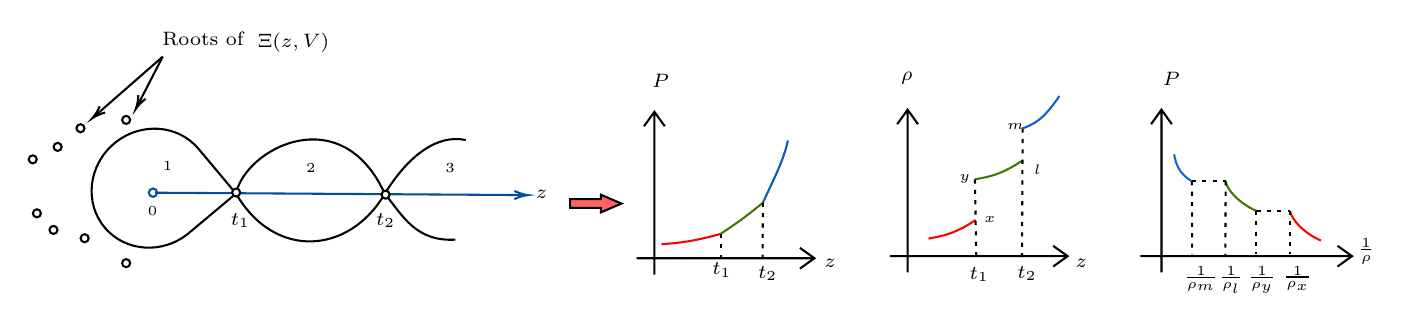
\begin{tikzpicture}[x=0.75pt,y=0.75pt,yscale=-1,xscale=1]
%uncomment if require: \path (0,372); %set diagram left start at 0, and has height of 372

%Shape: Boxed Bezier Curve [id:dp8816428801266158] 
\draw [color={rgb, 255:red, 255; green, 0; blue, 0 }  ,draw opacity=1 ]   (312,206.89) .. controls (319.57,206.12) and (325.54,205.99) .. (340.46,201.87) ;
%Shape: Axis 2D [id:dp16145854715037522] 
\draw  (300,213.59) -- (385.68,213.59)(308.57,143) -- (308.57,221.43) (378.68,208.59) -- (385.68,213.59) -- (378.68,218.59) (303.57,150) -- (308.57,143) -- (313.57,150)  ;
%Shape: Axis 2D [id:dp978316457425982] 
\draw  (422,212.59) -- (507.68,212.59)(430.57,142) -- (430.57,220.43) (500.68,207.59) -- (507.68,212.59) -- (500.68,217.59) (425.57,149) -- (430.57,142) -- (435.57,149)  ;
%Shape: Axis 2D [id:dp26039300590080416] 
\draw  (542.68,212.59) -- (644.68,212.59)(552.88,142) -- (552.88,220.43) (637.68,207.59) -- (644.68,212.59) -- (637.68,217.59) (547.88,149) -- (552.88,142) -- (557.88,149)  ;
%Shape: Boxed Bezier Curve [id:dp863718638776343] 
\draw [color={rgb, 255:red, 255; green, 0; blue, 0 }  ,draw opacity=1 ]   (440.66,204.11) .. controls (447.1,202.84) and (452.68,202.26) .. (463.34,195.19) ;
%Shape: Boxed Bezier Curve [id:dp4838128504636705] 
\draw [color={rgb, 255:red, 12; green, 107; blue, 216 }  ,draw opacity=1 ]   (559,163.55) .. controls (559.69,167.78) and (561.19,172.85) .. (567.56,176.52) ;
%Shape: Circle [id:dp11315515842109902] 
\draw   (30.12,150.94) .. controls (30.12,149.87) and (30.99,149) .. (32.06,149) .. controls (33.13,149) and (34,149.87) .. (34,150.94) .. controls (34,152.01) and (33.13,152.88) .. (32.06,152.88) .. controls (30.99,152.88) and (30.12,152.01) .. (30.12,150.94) -- cycle ;
%Shape: Circle [id:dp6787366031450796] 
\draw   (32.12,203.94) .. controls (32.12,202.87) and (32.99,202) .. (34.06,202) .. controls (35.13,202) and (36,202.87) .. (36,203.94) .. controls (36,205.01) and (35.13,205.88) .. (34.06,205.88) .. controls (32.99,205.88) and (32.12,205.01) .. (32.12,203.94) -- cycle ;
%Shape: Circle [id:dp7681830206540062] 
\draw   (52.12,146.94) .. controls (52.12,145.87) and (52.99,145) .. (54.06,145) .. controls (55.13,145) and (56,145.87) .. (56,146.94) .. controls (56,148.01) and (55.13,148.88) .. (54.06,148.88) .. controls (52.99,148.88) and (52.12,148.01) .. (52.12,146.94) -- cycle ;
%Shape: Circle [id:dp393998323220653] 
\draw   (52.12,215.94) .. controls (52.12,214.87) and (52.99,214) .. (54.06,214) .. controls (55.13,214) and (56,214.87) .. (56,215.94) .. controls (56,217.01) and (55.13,217.88) .. (54.06,217.88) .. controls (52.99,217.88) and (52.12,217.01) .. (52.12,215.94) -- cycle ;
%Shape: Circle [id:dp3591761889785463] 
\draw   (19.12,159.94) .. controls (19.12,158.87) and (19.99,158) .. (21.06,158) .. controls (22.13,158) and (23,158.87) .. (23,159.94) .. controls (23,161.01) and (22.13,161.88) .. (21.06,161.88) .. controls (19.99,161.88) and (19.12,161.01) .. (19.12,159.94) -- cycle ;
%Shape: Circle [id:dp448008178030871] 
\draw   (17.12,199.94) .. controls (17.12,198.87) and (17.99,198) .. (19.06,198) .. controls (20.13,198) and (21,198.87) .. (21,199.94) .. controls (21,201.01) and (20.13,201.88) .. (19.06,201.88) .. controls (17.99,201.88) and (17.12,201.01) .. (17.12,199.94) -- cycle ;
%Shape: Circle [id:dp8485667460597833] 
\draw   (9.12,191.94) .. controls (9.12,190.87) and (9.99,190) .. (11.06,190) .. controls (12.13,190) and (13,190.87) .. (13,191.94) .. controls (13,193.01) and (12.13,193.88) .. (11.06,193.88) .. controls (9.99,193.88) and (9.12,193.01) .. (9.12,191.94) -- cycle ;
%Shape: Circle [id:dp0935882432929589] 
\draw   (7.12,165.94) .. controls (7.12,164.87) and (7.99,164) .. (9.06,164) .. controls (10.13,164) and (11,164.87) .. (11,165.94) .. controls (11,167.01) and (10.13,167.88) .. (9.06,167.88) .. controls (7.99,167.88) and (7.12,167.01) .. (7.12,165.94) -- cycle ;
%Right Arrow [id:dp5160165324071785] 
\draw  [color={rgb, 255:red, 0; green, 0; blue, 0 }  ,draw opacity=1 ][fill={rgb, 255:red, 255; green, 0; blue, 0 }  ,fill opacity=0.61 ] (268,185.12) -- (282.81,185.12) -- (282.81,183) -- (292.68,187.24) -- (282.81,191.48) -- (282.81,189.36) -- (268,189.36) -- cycle ;
%Straight Lines [id:da40175091638638927] 
\draw    (71.68,116.48) -- (39.19,144.88) ;
\draw [shift={(37.68,146.2)}, rotate = 318.85] [color={rgb, 255:red, 0; green, 0; blue, 0 }  ][line width=0.75]    (6.56,-1.97) .. controls (4.17,-0.84) and (1.99,-0.18) .. (0,0) .. controls (1.99,0.18) and (4.17,0.84) .. (6.56,1.97)   ;
%Straight Lines [id:da42227604895998294] 
\draw    (71.68,116.48) -- (59.6,139.92) ;
\draw [shift={(58.68,141.7)}, rotate = 297.27] [color={rgb, 255:red, 0; green, 0; blue, 0 }  ][line width=0.75]    (6.56,-1.97) .. controls (4.17,-0.84) and (1.99,-0.18) .. (0,0) .. controls (1.99,0.18) and (4.17,0.84) .. (6.56,1.97)   ;
%Straight Lines [id:da403555006151344] 
\draw [draw opacity=0]   (178.68,169.5) -- (178.68,195.5) ;
%Shape: Rectangle [id:dp5158835307539544] 
\draw  [draw opacity=0] (64,169.72) -- (180.68,169.72) -- (180.68,194.5) -- (64,194.5) -- cycle ;
%Straight Lines [id:da34888006407657657] 
\draw [color={rgb, 255:red, 3; green, 76; blue, 160 }  ,draw opacity=1 ]   (68.01,182.01) -- (245.68,183.15) ;
\draw [shift={(247.68,183.17)}, rotate = 180.37] [color={rgb, 255:red, 3; green, 76; blue, 160 }  ,draw opacity=1 ][line width=0.75]    (6.56,-1.97) .. controls (4.17,-0.84) and (1.99,-0.18) .. (0,0) .. controls (1.99,0.18) and (4.17,0.84) .. (6.56,1.97)   ;
\draw [shift={(67,182)}, rotate = 0.37] [color={rgb, 255:red, 3; green, 76; blue, 160 }  ,draw opacity=1 ][line width=0.75]      (0, 0) circle [x radius= 2.01, y radius= 2.01]   ;
%Shape: Tear Drop [id:dp272851457137922] 
\draw   (84.37,201.37) .. controls (71.88,211.82) and (53.68,210.66) .. (43.72,198.77) .. controls (33.76,186.88) and (35.82,168.76) .. (48.31,158.3) .. controls (60.8,147.84) and (79,149) .. (88.96,160.9) .. controls (100.98,175.25) and (106.99,182.43) .. (106.99,182.43) .. controls (106.99,182.43) and (99.45,188.75) .. (84.37,201.37) -- cycle ;
%Curve Lines [id:da10060419654539787] 
\draw    (106.99,182.43) .. controls (111.68,160.63) and (157.68,136.63) .. (178.68,182.5) ;
%Curve Lines [id:da5863816426578047] 
\draw    (106.99,182.43) .. controls (125.68,214.63) and (161.68,211.63) .. (178.68,182.5) ;
%Curve Lines [id:da14753592564656481] 
\draw    (178.68,182.5) .. controls (189.68,164.63) and (203.68,153.63) .. (217.68,156.63) ;
%Curve Lines [id:da26991451847627657] 
\draw    (178.68,182.5) .. controls (187.68,193.58) and (193.68,205.58) .. (212.68,204.63) ;
%Shape: Circle [id:dp035910714470077876] 
\draw  [fill={rgb, 255:red, 255; green, 255; blue, 255 }  ,fill opacity=1 ] (105.12,181.94) .. controls (105.12,180.87) and (105.99,180) .. (107.06,180) .. controls (108.13,180) and (109,180.87) .. (109,181.94) .. controls (109,183.01) and (108.13,183.88) .. (107.06,183.88) .. controls (105.99,183.88) and (105.12,183.01) .. (105.12,181.94) -- cycle ;
%Shape: Circle [id:dp4309390960676185] 
\draw  [fill={rgb, 255:red, 255; green, 255; blue, 255 }  ,fill opacity=1 ] (177.12,182.94) .. controls (177.12,181.87) and (177.99,181) .. (179.06,181) .. controls (180.13,181) and (181,181.87) .. (181,182.94) .. controls (181,184.01) and (180.13,184.88) .. (179.06,184.88) .. controls (177.99,184.88) and (177.12,184.01) .. (177.12,182.94) -- cycle ;
%Curve Lines [id:da1800258159574435] 
\draw [color={rgb, 255:red, 65; green, 117; blue, 5 }  ,draw opacity=1 ]   (340.46,201.87) .. controls (349.68,195.72) and (353.68,192.72) .. (360.85,186.82) ;
%Shape: Boxed Bezier Curve [id:dp6921617703675862] 
\draw [color={rgb, 255:red, 65; green, 117; blue, 5 }  ,draw opacity=1 ]   (463,175.59) .. controls (469.44,174.31) and (475.02,173.73) .. (485.68,166.66) ;
%Curve Lines [id:da142472269960352] 
\draw [color={rgb, 255:red, 65; green, 117; blue, 5 }  ,draw opacity=1 ]   (583.77,176.52) .. controls (584.46,180.75) and (590.52,187.22) .. (598.62,190.79) ;
%Straight Lines [id:da7951881289244731] 
\draw  [dash pattern={on 1.5pt off 2.25pt}]  (340.46,201.87) -- (340.46,213.15) ;
%Straight Lines [id:da500933753036861] 
\draw  [dash pattern={on 1.5pt off 2.25pt}]  (463,175.59) -- (463.68,214.78) ;
%Straight Lines [id:da14975457152993088] 
\draw  [dash pattern={on 1.5pt off 2.25pt}]  (567.56,176.52) -- (583.77,176.52) ;
%Straight Lines [id:da1843463402056279] 
\draw  [dash pattern={on 1.5pt off 2.25pt}]  (583.77,176.52) -- (583.68,212.67) ;
%Straight Lines [id:da3624277033889689] 
\draw  [dash pattern={on 1.5pt off 2.25pt}]  (567.56,176.52) -- (567.68,211.67) ;
%Curve Lines [id:da2587872169692298] 
\draw [color={rgb, 255:red, 7; green, 91; blue, 189 }  ,draw opacity=1 ]   (360.85,186.82) .. controls (366.13,175.3) and (370.66,166.85) .. (372.93,156.87) ;
%Straight Lines [id:da9831398579139313] 
\draw  [dash pattern={on 1.5pt off 2.25pt}]  (360.85,186.82) -- (360.68,214.75) ;
%Shape: Boxed Bezier Curve [id:dp8024005479997904] 
\draw [color={rgb, 255:red, 12; green, 97; blue, 199 }  ,draw opacity=1 ]   (486,151.08) .. controls (491.02,148.85) and (495.37,147.83) .. (503.68,135.43) ;
%Straight Lines [id:da5086061427728615] 
\draw  [dash pattern={on 1.5pt off 2.25pt}]  (486,151.08) -- (485.68,213.32) ;
%Curve Lines [id:da6169340242913941] 
\draw [color={rgb, 255:red, 255; green, 0; blue, 0 }  ,draw opacity=1 ]   (614.83,190.79) .. controls (615.52,195.02) and (621.58,201.5) .. (629.68,205.07) ;
%Straight Lines [id:da6135488287955196] 
\draw  [dash pattern={on 1.5pt off 2.25pt}]  (598.62,190.79) -- (614.83,190.79) ;
%Straight Lines [id:da5610466287302585] 
\draw  [dash pattern={on 1.5pt off 2.25pt}]  (614.83,190.79) -- (614.83,211.55) ;
%Straight Lines [id:da4706916181477384] 
\draw  [dash pattern={on 1.5pt off 2.25pt}]  (598.62,190.79) -- (598.62,211.55) ;

% Text Node
\draw (306,123.4) node [anchor=north west][inner sep=0.75pt]  [font=\scriptsize]  {$P$};
% Text Node
\draw (426,122.4) node [anchor=north west][inner sep=0.75pt]  [font=\scriptsize]  {$\rho $};
% Text Node
\draw (646,202.4) node [anchor=north west][inner sep=0.75pt]  [font=\scriptsize]  {$\frac{1}{\rho }$};
% Text Node
\draw (510,212.4) node [anchor=north west][inner sep=0.75pt]  [font=\scriptsize]  {$z$};
% Text Node
\draw (389,212.4) node [anchor=north west][inner sep=0.75pt]  [font=\scriptsize]  {$z$};
% Text Node
\draw (552,122.4) node [anchor=north west][inner sep=0.75pt]  [font=\scriptsize]  {$P$};
% Text Node
\draw (63,187.4) node [anchor=north west][inner sep=0.75pt]  [font=\tiny]  {$0$};
% Text Node
\draw (116,103.4) node [anchor=north west][inner sep=0.75pt]  [font=\scriptsize]  {$\Xi ( z,V)$};
% Text Node
\draw (70,103) node [anchor=north west][inner sep=0.75pt]  [font=\scriptsize] [align=left] {Roots of };
% Text Node
\draw (250,179.4) node [anchor=north west][inner sep=0.75pt]  [font=\scriptsize]  {$z$};
% Text Node
\draw (70.31,165.46) node [anchor=north west][inner sep=0.75pt]  [font=\tiny]  {$\SR_{1}$};
% Text Node
\draw (139.31,166.7) node [anchor=north west][inner sep=0.75pt]  [font=\tiny]  {$\SR_{2}$};
% Text Node
\draw (206.31,166.7) node [anchor=north west][inner sep=0.75pt]  [font=\tiny]  {$\SR_{3}$};
% Text Node
\draw (103,190.4) node [anchor=north west][inner sep=0.75pt]  [font=\scriptsize]  {$t_{1}$};
% Text Node
\draw (173,190.4) node [anchor=north west][inner sep=0.75pt]  [font=\scriptsize]  {$t_{2}$};
% Text Node
\draw (335,214.4) node [anchor=north west][inner sep=0.75pt]  [font=\scriptsize]  {$t_{1}$};
% Text Node
\draw (466,191.81) node [anchor=north west][inner sep=0.75pt]  [font=\tiny]  {$x$};
% Text Node
\draw (454,171.68) node [anchor=north west][inner sep=0.75pt]  [font=\tiny]  {$y$};
% Text Node
\draw (610,215.9) node [anchor=north west][inner sep=0.75pt]  [font=\tiny]  {$\frac{1}{\rho _{x}}$};
% Text Node
\draw (357,215.87) node [anchor=north west][inner sep=0.75pt]  [font=\scriptsize]  {$t_{2}$};
% Text Node
\draw (490,167.3) node [anchor=north west][inner sep=0.75pt]  [font=\tiny]  {$l$};
% Text Node
\draw (477,147.17) node [anchor=north west][inner sep=0.75pt]  [font=\tiny]  {$m$};
% Text Node
\draw (593,216.1) node [anchor=north west][inner sep=0.75pt]  [font=\tiny]  {$\frac{1}{\rho _{y}}$};
% Text Node
\draw (579,216.1) node [anchor=north west][inner sep=0.75pt]  [font=\tiny]  {$\frac{1}{\rho _{l}}$};
% Text Node
\draw (562,216.1) node [anchor=north west][inner sep=0.75pt]  [font=\tiny]  {$\frac{1}{\rho _{m}}$};
% Text Node
\draw (459,216.4) node [anchor=north west][inner sep=0.75pt]  [font=\scriptsize]  {$t_{1}$};
% Text Node
\draw (482,215.87) node [anchor=north west][inner sep=0.75pt]  [font=\scriptsize]  {$t_{2}$};


\end{tikzpicture}
